%!TEX program = xelatex
\documentclass[11pt, a4paper, titlepage]{article}

\usepackage{amsmath}
\usepackage{amssymb}

% fonts
% \usepackage{xeCJK}
% \setCJKmainfont[BoldFont=SimHei]{SimSun}
% \setCJKfamilyfont{hei}{SimHei}
% \setCJKfamilyfont{kai}{KaiTi}
% \setCJKfamilyfont{fang}{FangSong}
% \newcommand{\hei}{\CJKfamily{hei}}
% \newcommand{\kai}{\CJKfamily{kai}}
% \newcommand{\fang}{\CJKfamily{fang}}
%
\usepackage[UTF8,heading=false,scheme=plain]{ctex}
% style
\usepackage[top=2.54cm, bottom=2.54cm, left=3.18cm, right=3.18cm]{geometry}
\linespread{1.5}
\usepackage{indentfirst}
\parindent 2em
\punctstyle{quanjiao}
\renewcommand{\today}{\number\year 年 \number\month 月 \number\day 日}

% figures and tables
\usepackage{graphicx}
\usepackage[font={bf, footnotesize}, textfont=md]{caption}
\makeatletter
    \newcommand\fcaption{\def\@captype{figure}\caption}
    \newcommand\tcaption{\def\@captype{table}\caption}
\makeatother
\usepackage{booktabs}
\renewcommand\figurename{图}
\renewcommand\tablename{表}
\newcommand{\fref}[1]{\textbf{图 \ref{#1}}}
\newcommand{\tref}[1]{\textbf{表 \ref{#1}}}
\newcommand{\tabincell}[2]{\begin{tabular}{@{}#1@{}}#2\end{tabular}} % multiply lines in one grid
\usepackage{longtable} % long table

\usepackage{listings}
\lstset{basicstyle=\ttfamily}

\usepackage{xcolor}
\renewcommand{\r}{\color{red}}
\usepackage{tabulary}
\usepackage{url}
\usepackage{hyperref}

% start of document
\title{\textbf{简易版“微信”实验报告}}
\author{
    丁雨晖 \quad 计54 \quad 2015010866
}
\date{\today}

% -----------------start here------------------%
\begin{document}

\maketitle

\newpage

\section{实验原理}
本次实验采用客户端-服务器架构,基于Linux系统使用socket编程技术实现了一个简易版的即时通信软件。客户端、服务器程序的开发语言均为C语言。
服务器使用多线程并发地处理多个客户端的通信请求,客户端程序也使用不同的线程分别进行接收和发送数据的操作。服务器作为整个系统的中心,维护着所
有用户的状态信息,在不同的用户与socket标识符之间建立了一一对应关系,以对客户端之间的通信提供转发。
\section{亮点}
本次实验中服务器和客户端均使用pthread实现了多线程,服务器使用多线程与多个不同的客户端进行连接,客户端使用多线程分别进行接收和发送数据的
操作。由于服务器维护着所有用户的信息,被所有线程所共享,因此在服务器端使用了互斥锁pthread\_mutex,不允许多个线程同时对用户信息进行修改,
这样就避免了不同线程之间可能出现的不同步问题。
\section{实现细节}
\subsection{用户管理}
系统支持客户端程序进行用户注册、登录、查询联系人、添加好友等操作。客户端以一定格式向服务器发送请求,服务器端在自己存储的用户状态信息中进行查询,并返回相应的结果。

\subsection{消息收发}
消息收发的过程比较简单,服务器在其中仅仅充当了中转的角色,将来自发送方的消息通过与接收方连接的socket发送给接收方。服务器在用户信息中同时记录
了用户当前的通信状态,例如是否处于聊天模式,与哪位用户进行聊天等等。在客户端,为了实现通信的即时性,分离了接收和发送的功能,交由不同的线程各自
实现。

\subsection{文件收发}
文件收发的过程与消息收发类似,但文件的规模一般较大,无法一次性传输完毕。我采用了分段传输的方法,每次传送一个缓冲区的大小,即2KB。在文件传输开始
之前,会先发送一定格式的消息通知对方即将开始的文件传输过程,这一消息中包含了所要传输的文件大小(字节数),以便接收方判断何时文件接收完毕。经验证
可以成功传输200MB以上大小的文件

\subsection{离线消息、文件收发}
对于离线消息,服务器会将其保存,待收到recvmsg请求后再发送给相应的接收方;对于离线文件,服务器会保存其文件名,并将传输来的文件暂存在本地。收到
收到recvfile请求后,服务器会先发送暂存的文件名,用户指定接收某一文件后才会开始实际的文件传输。

检查时未演示离线消息、文件收发功能,下面提供几张效果截图:

\begin{center}
    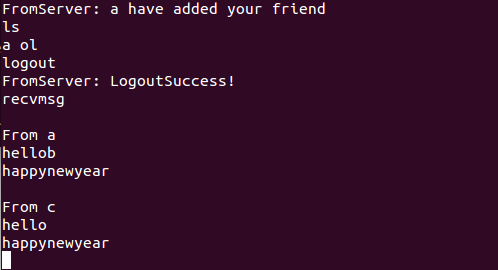
\includegraphics[width=13cm]{image/recvmsg.png}
    \fcaption{recvmsg效果图}
\end{center}

\begin{center}
    
\includegraphics[width=13cm]{image/recvfile.png}
    \fcaption{recvfile效果图}
\end{center}

\section{思考问题}
\subsection{Linux系统里Socket与文件的关系}
Linux系统中文件与Socket均由一个描述符来表示,调用read和write方法进行读写操作时二者并无区别(内部实现使用了多态),可认为Socket是一种特殊的文件。

\subsection{即时通信时服务器程序的角色}
在本次实验中,服务器是整个系统的中心,不仅负责与客户端应用程序建立连接,同时客户端之间消息、数据的传输都需要经过服务器进行转发。

\subsection{服务器端口与客户端连接个数的关系}
我认为服务器端口与客户端连接个数并无联系,本次实验中我的服务器监听端口号为固定值8888,而这一端口可以连接多个客户端。服务器所能与客户端建立
的连接个数确实是有限的,但这应受限于服务器系统的性能,与服务器的端口号无关。

\end{document}